\section{Symmetry}

As recently noted by \cite{Caselles-Dupre2019}, ...


\hypertarget{cart-pole}{%
\subsubsection{Cart pole}\label{cart-pole}}

\hypertarget{mirror-symmetry}{%
\paragraph{Mirror symmetry}\label{mirror-symmetry}}

\begin{figure}
\centering
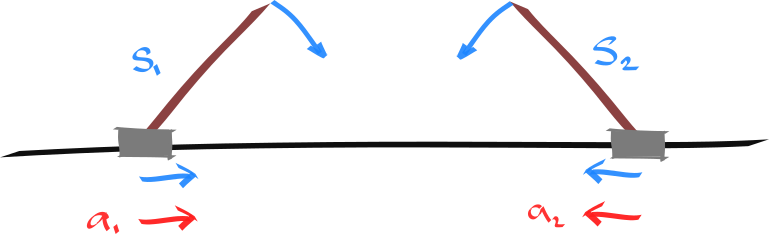
\includegraphics[width=1\textwidth,height=0.25\textheight]{../../pictures/drawings/cart-pole-mirror.png}
\caption{???}
\end{figure}

\begin{align}
\Delta_{\tau}(s, a) = \mathop{\mathbb E}_{s' \sim p(\cdot| s, a)} (s' - s) \\
\Delta_{\tau}(s_1, a_1) = - \Delta_{\tau}(s_2, a_2) \\
\end{align}

(\emph{this assumes we have a `nice' state representation where
differenes make sense})

\begin{align}
\Delta_{T}(s, a) = (T \circ Q)(s,a) - Q(s,a)\\
\Delta_{T}(s_1, a_1) = \Delta_{T}(s_2, a_2) \\
\end{align}

The expected value is conserved between the pair (assuming we have a
policy with mirror symmetry).

\begin{align}
\text{ set}\;\;\pi(a | s) = \pi(-a| -s) \\
Q_\pi(s_1, a_1) = Q_\pi(s_2, a_2) \\
Q_\pi(s_1, a_2) = Q_\pi(s_2, a_1) \\
\end{align}

The (discounted) reachable rewards are conserved between the pair. (!!!)

\begin{align}
\{r(s, a, s'): \forall s \in \mathcal R(s_1, a_1)\} = \{r(s, a, s'): \forall s \in \mathcal R(s_2, a_2)\}
\end{align}


\hypertarget{translational-symmetry}{%
\paragraph{Translational symmetry}\label{translational-symmetry}}

\begin{figure}
\centering
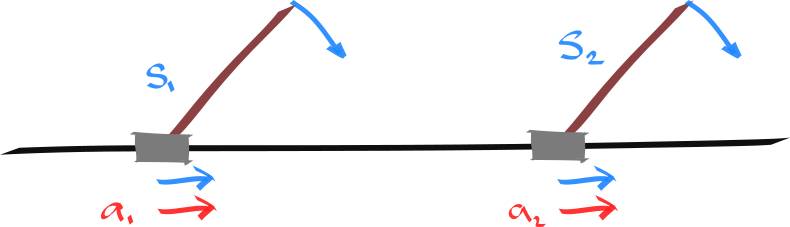
\includegraphics[width=1\textwidth,height=0.25\textheight]{../../pictures/drawings/cart-pole-translation.png}
\caption{???}
\end{figure}

(special case of regular actions)


\begin{align}
\Delta_{\tau}(s_1, a_1) = \Delta_{\tau}(s_1, a_2) = \Delta_{\tau}(s_2, a_1) = \Delta_{\tau}(s_2, a_2) \\
 \text{ if} \;\;\forall a\;\;\pi(a | s_1) = \pi(a| s_2) \\
Q_\pi(s_1, a_1) = Q_\pi(s_2, a_2)= Q_\pi(s_1, a_2) = Q_\pi(s_2, a_1) \\
\end{align}


\hypertarget{local-symmetry}{%
\subsubsection{Local symmetry}\label{local-symmetry}}

(\emph{this is approximately a symmetry})

\begin{figure}
\centering
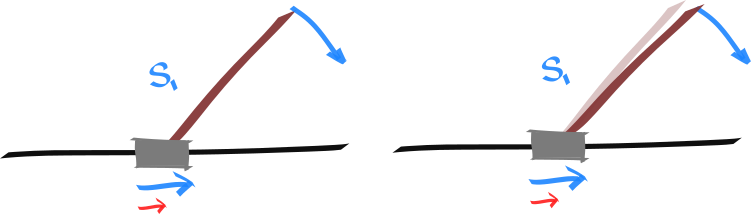
\includegraphics[width=1\textwidth,height=0.25\textheight]{../../pictures/drawings/cart-pole-approx.png}
\caption{???}
\end{figure}

\begin{align}
\Delta(s_1, a_1) = \Delta(s_1, a_2) = \Delta(s_2, a_1) = \Delta(s_2, a_2) \\
\forall a \text{ set}\;\;\pi(a | s_1) = \pi(a| s_2) \\
Q_\pi(s_1, a_1) \approx Q_\pi(s_2, a_2)  \\
\end{align}

\hypertarget{future-translational-symmetry}{%
\subsubsection{Future translational
symmetry}\label{future-translational-symmetry}}

\begin{figure}
\centering
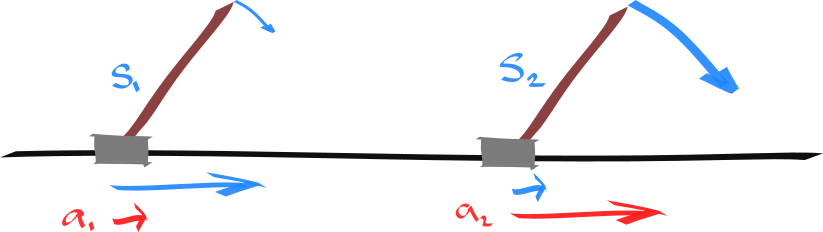
\includegraphics[width=1\textwidth,height=0.25\textheight]{../../pictures/drawings/cart-pole-state.png}
\caption{???}
\end{figure}

different states, different actions. but maps into translational
symmetry.

After this action. All future actions will have the same effect. In this
sense, these two state-actions are similar.

\begin{align}
\forall a: \mathop{\mathbb E}_{s' \sim p(\cdot| s_1, a_1)} [\Delta(s', a)] =  \mathop{\mathbb E}_{s' \sim p(\cdot| s_2, a_2)} [\Delta(s', a)] \\
\end{align}

\hypertarget{temporal-mirror-symmetry}{%
\paragraph{Temporal mirror symmetry}\label{temporal-mirror-symmetry}}

This is simply a result of the earlier mirror symmetry?!? (want to show
this!)

permutations of actions that yield similar outcomes.

\begin{figure}
\centering
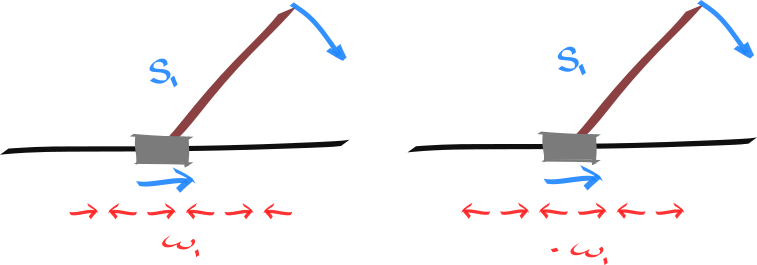
\includegraphics[width=1\textwidth,height=0.25\textheight]{../../pictures/drawings/cart-pole-temporal-mirror.png}
\caption{???}
\end{figure}

\begin{align}
p(s'|s, \omega) = \prod p(s|s, a)\omega(a|s) \\
p(\cdot|s_1, \omega_1) = p(\cdot|s_1, -\omega_1) \\
Q_{\pi}(s_1, \omega_1) = Q_{\pi}(s_1,-\omega_1) \\
\end{align}

\hypertarget{temporal-symmetry}{%
\paragraph{Temporal symmetry}\label{temporal-symmetry}}

\begin{figure}
\centering
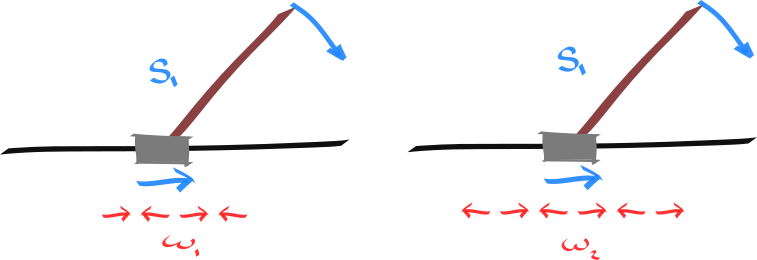
\includegraphics[width=1\textwidth,height=0.25\textheight]{../../pictures/drawings/cart-pole-temporal-approx.png}
\caption{???}
\end{figure}

\begin{align}
p(\cdot|s_1, \omega_1) = p(\cdot|s_1, \omega_2) \\
Q_{\pi}(s_1, \omega_1) = Q_{\pi}(s_1,\omega_2) \\
\end{align}

\hypertarget{pong}{%
\subsubsection{Pong}\label{pong}}

\hypertarget{mirror-symmetry-vertical}{%
\paragraph{Mirror symmetry (vertical)}\label{mirror-symmetry-vertical}}

\begin{figure}
\centering
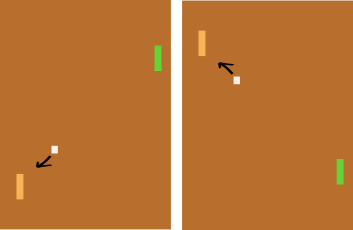
\includegraphics[width=1\textwidth,height=0.25\textheight]{../../pictures/drawings/pong-vert-flip.png}
\caption{???}
\end{figure}

(\emph{how can a change in state be evaluated? we need a
representation\ldots{}})

\begin{align}
\Delta_{T}(s, a) = (T \circ Q)(s,a) - Q(s,a)\\
\Delta_{T}(s_1, a_1) = \Delta_{T}(s_2, a_2) \\
\end{align}

\begin{align}
\forall a \text{ set}\;\;\pi(a | s_1) = \pi(-a| s_2) \\
Q_\pi(s_1, a_1) = Q_\pi(s_2, a_2) \\
Q_\pi(s_1, a_2) = Q_\pi(s_2, a_1) \\
\end{align}

\hypertarget{mirror-symmetry-horizontal}{%
\paragraph{Mirror symmetry
(horizontal)}\label{mirror-symmetry-horizontal}}

\begin{figure}
\centering
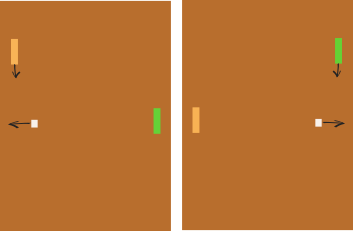
\includegraphics[width=1\textwidth,height=0.25\textheight]{../../pictures/drawings/pong-horz-flip.png}
\caption{???}
\end{figure}

Upon pretending to play as your opponent (flipping the image and
inverting the colors, via \(\rho: O \to O\), and ??? the actions)

\begin{align}
Q(s_1, a_1) = - V(\rho(s_2)) \\
\end{align}

(\emph{this really requires you to disentangle the model from your
opponent!?})

\begin{align}
\tau(s'|s, a_{p=0}) &= f_{p=0}(s''|s, a) \cdot f_{p=1}(s'|s'', \hat a) \cdot \pi_{p=1}(\hat a|s'') \\
Q_{p=0}(s, a) &= -Q_{p=1}(s, a)
\end{align}

\hypertarget{translational-symmetry-1}{%
\paragraph{Translational symmetry}\label{translational-symmetry-1}}

\begin{figure}
\centering
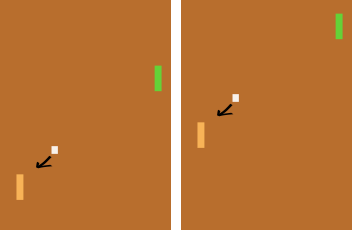
\includegraphics[width=1\textwidth,height=0.25\textheight]{../../pictures/drawings/pong-trans.png}
\caption{???}
\end{figure}

(\emph{although there are boundary cases which cannot be ignored. how
can they be dealt with!?})

\begin{align}
\forall a: Q_{\pi_1}(s_1, a) = Q_{\pi_2}(s_2, a) \\
\forall a, t: \pi_1(a|s^t_{s^0=s_1}) = \pi_2(a|s^t_{s^0=s_2})
\end{align}

If we take the same actions, in translated states, we get the same
outcome (up to the boundary conditions).

\hypertarget{temporal-symmetries}{%
\paragraph{Temporal symmetries}\label{temporal-symmetries}}

\begin{figure}
\centering
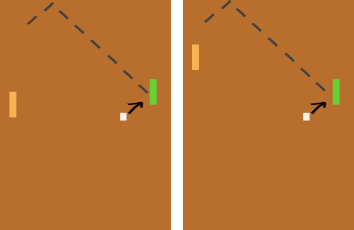
\includegraphics[width=1\textwidth,height=0.25\textheight]{../../pictures/drawings/pong-reach.png}
\caption{???}
\end{figure}

\begin{align}
\exists \pi_1, \pi_2 \;\;\text{s.t.} \;\; Q^{\pi_1}(s_1, a_1) = Q^{\pi_2}(s_2, a_2)
\end{align}

The same future state can be reached, and thus the same rewards can be
achieved.


\subsection{n-dimensional Cart pole}

So, how can we test a learners ability to detect symmetries and exploit them?
We propose a simple test, the n-dimensional cart pole.

% insert image

Many people realise that this problem can be reduce to n, one dimensional cart pole problems.
But the learner needs to infer that.
